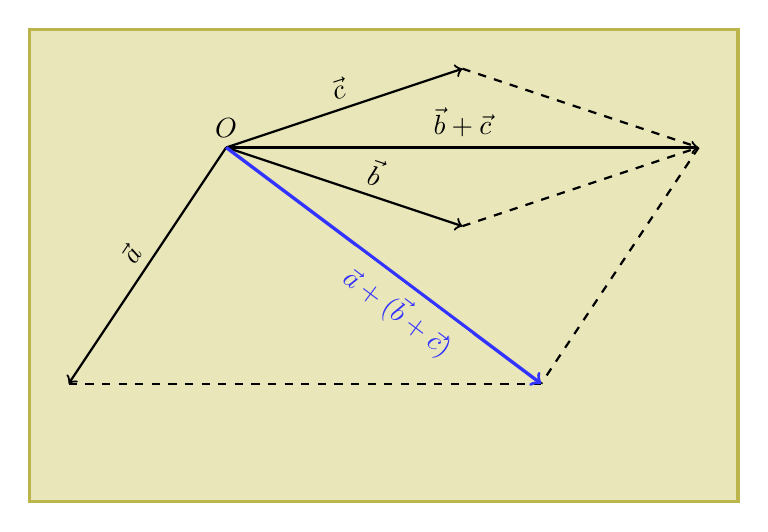
\begin{tikzpicture}
  \draw[draw = olive!60, fill = olive!20, very thick]
    (-2.5, -4.5) rectangle (6.5, 1.5);

  \draw[dashed, thick] (3, 1) -- (6, 0);
  \draw[dashed, thick] (3, -1) -- (6, 0);
  \draw[dashed, thick] (-2, -3) -- (4, -3);
  \draw[dashed, thick] (6, 0) -- (4, -3);

  \draw[->, thick] (0, 0) -- (-2, -3)
    node[midway, above, sloped] {\(\vec{a}\)};
  \draw[->, thick] (0, 0) -- (3, -1)
    node[pos = 0.6, above, sloped] {\(\vec{b}\)};
  \draw[->, thick] (0, 0) -- (3, 1)
    node[midway, above, sloped] {\(\vec{c}\)};

  \draw[->, thick] (0, 0) -- (6, 0)
    node[midway, above] {\(\vec{b} + \vec{c}\)};
  \draw[->, very thick, color = blue!80] (0, 0) -- (4, -3)
    node[pos = 0.6, below, sloped, fill = olive!20]
    {\textcolor{blue!80}{\(\vec{a} + (\vec{b} + \vec{c})\)}};
  
  \draw (0, 0) node[above] {\(O\)};
  \point{0, 0};
\end{tikzpicture}